\documentclass[12pt, a4paper]{article}
\usepackage[utf8]{inputenc}
\usepackage{amsmath, amssymb, amsthm}
\usepackage[margin=2.5cm]{geometry}
\usepackage{enumitem}
\usepackage[utf8]{inputenc}
\usepackage[T1]{fontenc}
\usepackage{amsmath, amssymb, amsthm}
\usepackage{mathtools}
\usepackage{geometry}
\usepackage{setspace}
\usepackage{booktabs}
\usepackage{array}
\usepackage{bm}
\usepackage{multirow}
\usepackage{caption}
\usepackage{graphicx}
\usepackage{tikz}
\usetikzlibrary{arrows.meta, positioning, calc}
\usepackage{hyperref}
\usepackage[round]{natbib}
\usepackage{xcolor}
\usepackage{longtable}
\usepackage{float}
\usepackage{tcolorbox}
\newcolumntype{P}[1]{>{\raggedright\arraybackslash}p{#1}}
\usepackage{pdflscape}
\usepackage{caption}


\geometry{margin=2.5cm}

\newtheorem{assumption}{Assumption}
\newtheorem{proposition}{Proposition}
\newtheorem{corollary}{Corollary}
\newtheorem{lemma}{Lemma}
\newtheorem{definition}{Definition}
\newtheorem{remark}{Remark}

\title{The Economics of illicit Drug Demand}
\author{Draft --- Work in Progress}
\date{}

\begin{document}

\maketitle

\vspace{1cm} % Ein bisschen Abstand zwischen dem Titelblock und dem Zitat

\begin{center}
    \textit{,,Si no hubiera consumo, no habría ventas."} \\
    \vspace{0.2cm} % Kleiner Abstand zwischen den Sprachen
    \textit{,,If there were no consumption, there would be no sales."} \\
    \vspace{0.5cm}
    --- Joaquín ,,El Chapo`` Guzmán
\end{center}

\newpage % Nutze dies, wenn das Zitat allein auf dem Titelblatt stehen soll

% Hier beginnt dann dein eigentliches Inhaltsverzeichnis oder der Text...
\noindent As this is a clear naive correlation --- potentially confounded by tourism, urbanisation, income, and other city-level characteristics --- I propose an instrumental variable strategy that generates exogenous variation in access to mobile internet and therefore in the use of the smartphone-based platforms described above. For instance, European countries auctioned 4G spectrum between 2011 and 2015, with auction dates determined by regulatory and political processes unrelated to local drug consumption. Within countries, the speed of the subsequent network roll out varied with local geography: flatter cities received coverage faster because base station signals propagate further in flat terrain, reducing the infrastructure cost per capita. I exploit this by interacting the Terrain Ruggedness Index (TRI) in a 20km radius around each city with a post-4G-auction indicator, generating city-level variation in mobile internet access that is plausibly exogenous to drug demand. This identification strategy follows the logic established by \citet{falck_2014}, who exploit historical peculiarities of the German voice telephony network --- specifically, the quasi-random distance of municipalities to their main distribution frame --- to generate exogenous variation in availability. A broader set of candidate instruments is shown in the Appendix in Table~\ref{tab:instruments}. 

A potential limitation of this strategy is that it instruments access to mobile internet rather than platform use directly, and therefore cannot isolate the specific channel through which the effect operates. To directly test whether online drug market platforms are the operative mechanism, I propose to complement the IV design with event studies exploiting high-frequency wastewater data. While the SCORE data covers a large number of cities, it is collected during only one campaign week per year, limiting the ability to detect short-run disruptions. However, high-frequency wastewater monitoring exists for selected countries and cities over extended time periods.\footnote{Switzerland (EAWAG/DroMedArio): 10 cities with continuous monitoring since 2021, samples every 13 days; United Kingdom (Home Office WWAP): $\sim$50 sites since May 2021; and individual research laboratories in Barcelona, Milan, Antwerp, and Oslo with varying coverage.} This data can be used to perform event studies around sharp disruptions to online drug markets --- such as the arrest of Telegram founder Pavel Durov in August 2024, which temporarily disrupted the trust in encrypted drug-selling channels, or the COVID-19 lockdowns, which simultaneously eliminated street-level dealing while leaving digital channels intact. If consumption drops sharply when a major platform is disrupted but recovers as users migrate to alternatives, this would constitute direct evidence for the platform mechanism that the IV design alone cannot provide. Together, the two strategies are complementary: the IV estimates the causal effect of the enabling infrastructure, while the event studies try to isolate specific channels.\footnote{Additional candidate events are discussed in the Appendix.}
%%%%%

\section{The Wrong Side of Disruption: How Digital Innovation Reduced Drug Market Frictions and Fuelled Consumption}

%\title{Fighting Supply, Losing to Demand: How Digital Platforms Reduced Drug Market Frictions and Fuelled the European Drug Boom}
%\section{\title{Delivered to Your Door: How Mobile Internet Fuelled the European Drug Boom}}

%\title{Disrupting the Drug Market: Mobile Internet, Frictions, and Consumption}

%\title{Swipe, Order, Consume: How Mobile Internet Reduced Market Frictions and Fuelled Drug Consumption in Europe}

The ``War on Drugs,'' launched by President Nixon in 1971, more than fifty years ago, seems to be lost. In the United States, drug-related deaths have become the number one cause of death for adults under 45, with over 100,000 fatalities per year, mainly due to deadly opioids. While the opioid crisis is largely concentrated in North America, the consumption of hard drugs is soaring globally. In Switzerland, cocaine consumption has more than doubled since 2012 according to wastewater analyses \citep{wastewater_2026}; among young adults in Zurich, nearly one in four has consumed cocaine at least once \citep{quednow_uzh_2025}; new psychoactive substances are flooding the market; and the overall trend is upward across Europe, where cocaine loads in wastewater have nearly tripled since 2012 \citep{wastewater_2026}. The trend extends well beyond Europe: in Africa, overall drug consumption is projected to increase by 40\% by 2026 \citep{africa_2025}, and Southeast Asia is experiencing an unprecedented methamphetamine crisis \citep{asia_2025}. The associated costs are staggering: in the United States alone, they are estimated at around one trillion USD per year, not counting costs like the value of statistical lives lost, the destabilization of entire nations, or the opportunity costs of mass incarceration \citep{ncdas_2025, whitehouse_opioid_2025}. Yet despite international cooperation among authorities to target the highly concentrated production and supply of drugs --- leading to record seizures every year, global spending on drug enforcement exceeding 100 billion USD per annum \citep{count_costs_2013}, and unprecedented capabilities in surveillance and public awareness --- drug prices have fallen, purity has increased, and consumption has surged. In a report published in 2014, followed by another in 2016, signed by five Nobel laureates in Economics, including Kenneth Arrow and Oliver Williamson, the authors concluded:

\begin{quote}
\textit{``The strategy has failed based on its own terms. Evidence shows 
that drug prices have been declining while purity has been increasing 
[\ldots] despite drastic increases in global enforcement spending. It is 
time to end the `war on drugs' and massively redirect resources towards 
effective evidence-based policies underpinned by rigorous economic 
analysis.''} \citep{lse_2014}
\end{quote}

\noindent The scientific literature strongly supports this conclusion. \citet{pollack_reuter_2014} find little evidence that raising the risk of arrest, incarceration, or seizure at any level of the distribution system raises retail prices. \citet{caulkins_reuter_taylor_2006} go further, showing that cocaine and heroin prices have fallen substantially during a period of massive increases in enforcement. The data confirm this pattern: in Europe, the nominal street price of a gram of cocaine has remained roughly stable over the past 15 to 20 years, while purity has increased markedly (30-45\% since 2013) --- meaning consumers now obtain a stronger product for the same price \citep{euda_europol_cocaine_2022}, a finding consistent with the systematic audit of international drug surveillance systems by \citet{werb_2011_violence}. Given the growing consensus that supply-side enforcement has failed to curb drug consumption, the need for fundamentally different policy approaches has become increasingly urgent. 

\noindent A good starting point may be to listen to the driving forces of this global epidemic themselves. As Joaqu\'{i}n ``El Chapo'' Guzm\'{a}n, once the world's most powerful drug trafficker, put it: \textit{``If there was no consumption, there would be no 
sales.''}\footnote{When asked about his responsibility for global drug consumption, Guzm\'{a}n responded: \textit{``If there was no consumption, there would be no sales. It is true that consumption, day after day, becomes bigger and bigger. So it sells and sells.''} 
See \citet{penn_elchapo_2016}.}. 

If supply consistently exceeds demand, then consumption is ultimately determined by the buyer's decision to seek out and purchase a substance. For opioids, this decision is largely driven by physiological dependence --- sellers only need to ``hook'' the consumer, and demand becomes highly inelastic. But for other drugs like cocaine, MDMA, ketamine, cannabis or amphetamine, the picture is more complex: these substances carry significant addiction potential, yet a substantial share of consumption is recreational, occasional, and discretionary. \citet{galenianos_2012} argue that retail drug markets do not operate according to Walrasian principles. The dominant frictions are search costs and moral hazard: buyers cannot observe purity before purchase and must invest time and accept risk to find a seller. In this framework, it is not the monetary price alone that determines consumption, but the total cost of locating, evaluating, and completing a transaction. In a follow-up paper, \citet{galenianos_2017} structurally estimate this model using US crack cocaine data. They find that eliminating moral hazard --- making purity observable --- would increase average purity by 20\%, reduce purity dispersion by 80\%, and raise the number of active buyers by 7\%, leading to an approximately 12\% increase in aggregate consumption. This implies that demand-side reductions in search frictions expand both market participation and individual consumption, while increases in these frictions have the opposite effect.\footnote{See \citet{galenianos_2017}, Table 4, and \citet{galenianos_2012}, Proposition 7.}  This finding is exactly aligned with the observed increase in purity of drugs as well as the increase in consumption in Europe.

This raises the question of whether a broader change in market frictions could be driving the global increase in drug consumption. Studying this question could not only provide insights into the economics of illicit drug markets, but also help identify more nuanced, demand-centred policy interventions that successfully reduce drug consumption and the corresponding economic and social costs.

Analyzing the structure of the illicit drug market over the last fifteen years, it becomes clear that it has changed fundamentally. As Boris Quednow, a leading addiction researcher at the University of Zurich, summarized: \textit{``In the past, people had to seek out shady dealers; today, drugs can be ordered contact-free via social media or messenger services and delivered within minutes.''} \citep{quednow_uzh_2025}. While darknet markets first 
demonstrated that drugs could be traded online, the market has since evolved well beyond the dark web. On Snapchat, Instagram, and other social media platforms, dealers advertise openly using coded emojis and hashtags --- operating with high efficiency, supported by platform algorithms that actively recommend new dealer profiles to users \citep{demant_emcdda_2023}.\footnote{In a netnographic study commissioned by the EMCDDA, a newly created user 
profile identified and connected with multiple active cocaine dealers within a single day, and was offered a position as a delivery driver within a week \citep{demant_emcdda_2023}.} Encrypted messaging apps like Telegram host dedicated drug-selling groups with administrator-enforced rules, review systems, and automated bots --- organizational structures that closely resemble legitimate e-commerce \citep{dewey_2024_telegram}. Payment is made in cash or cryptocurrency, and the drugs are delivered directly to the buyer by courier, taxi, or food delivery driver --- often within minutes \citep{demant_emcdda_2023, moyle_2019_drugsforsale}.


\noindent Each of these channels reduces a distinct component of the buyer's total cost of consumption. Social media and messaging apps dramatically lower search costs by enabling buyers to identify and contact sellers anonymously within hours. At the same time, online reputation systems, vendor ratings, and escrow services mitigate the moral hazard problem that \citet{galenianos_2017} identify as the second dominant friction in retail drug markets, making product quality partially observable before purchase.\footnote{\citet{bhaskar_2019} show that on darknet platforms, these mechanisms reduce quality dispersion below street-market levels.}All of these channels operate primarily through smartphones and none of these channels existed in their current form fifteen years ago.\footnote{The iPhone was introduced in 2008, WhatsApp in 2009, Instagram in 2010, Snapchat in 2011, Telegram in 2013, and the first major darknet market (Silk Road) operated from 2011 to 2013. European 4G networks began rolling out between 2011 and 2015, making mobile internet fast enough to support these platforms ubiquitously what is also seen in the explosion of usage of those platforms in the years after.}

The diffusion of mobile internet across Europe between 2011 and 2016, the corresponding rise of the platforms described 
above, the theoretical framework linking search frictions to consumption, and the observed surge in drug use together provide a unique opportunity to study what drives the demand for illicit drugs. Europe is particularly well suited for this analysis: unlike the United States, its drug market is 
not confounded by the fentanyl crisis, and the SCORE wastewater network provides objective, population-level consumption measures. Using this data from up to 168 European cities with varying year coverage, Figure~\ref{fig:binscatter} plots cocaine loads against internet penetration, revealing a clear positive within-city relationship.

\begin{figure}[H]
    \centering
    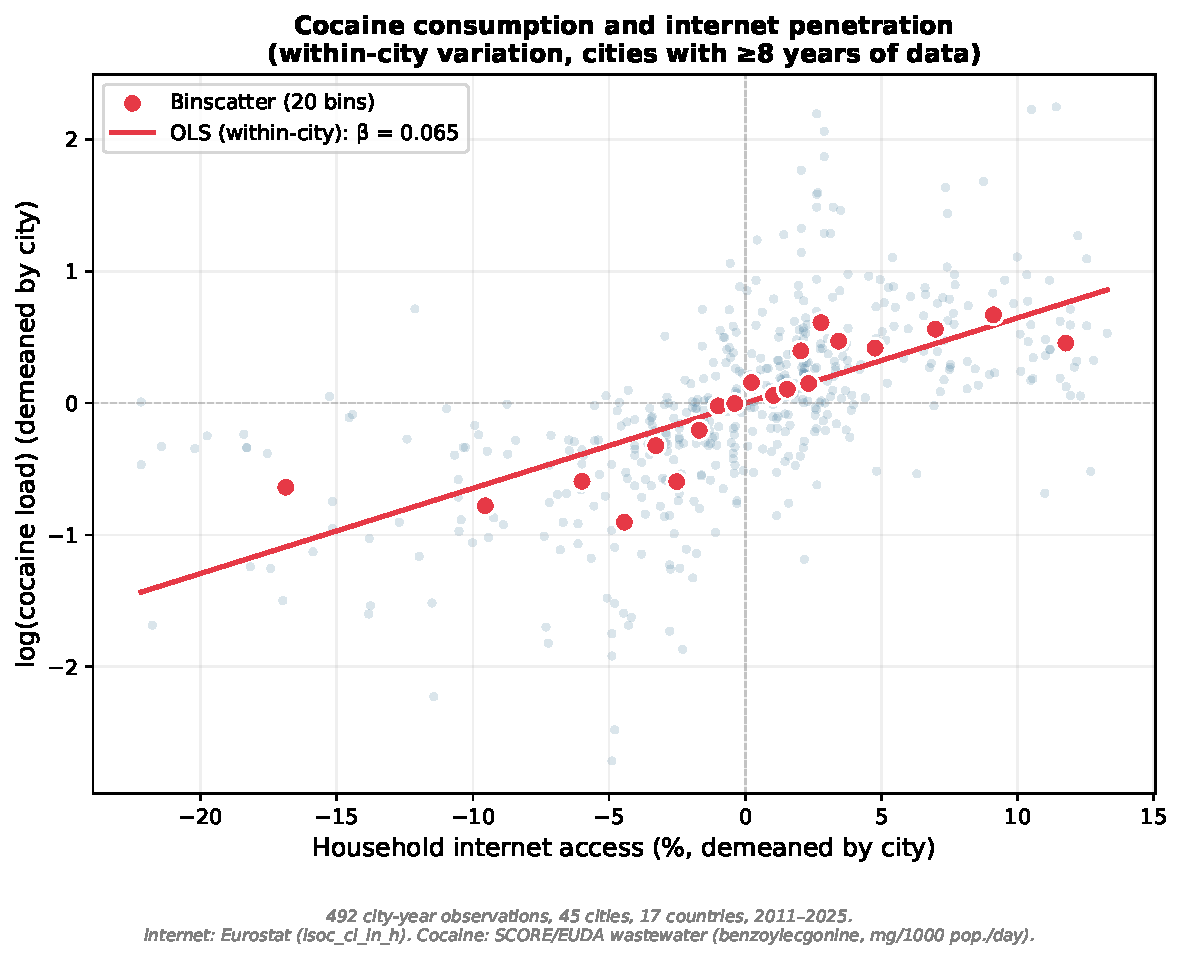
\includegraphics[width=0.45\textwidth]{fig_binscatter_final.pdf}
    \captionsetup{font=scriptsize}
    \caption{Within-city correlation between internet penetration 
    and cocaine consumption. Both variables are demeaned by city. 
    Red dots show a binscatter with 20 equal-sized bins. The 
    sample includes 45 European cities with at least 10 years of 
    observations. Internet access: Eurostat, percentage of 
    households. Cocaine: SCORE/EUDA wastewater data.}
    \label{fig:binscatter}
\end{figure}

\noindent As this is a clear naive correlation --- potentially confounded by tourism, urbanisation, income, and other city-level characteristics --- I propose an instrumental variable strategy that generates exogenous variation in access to mobile internet and therefore in the use of the smartphone-based platforms described above. For instance, European countries auctioned 4G spectrum between 2011 and 2015, with auction dates determined by regulatory and political processes unrelated to local drug consumption. Within countries, the speed of the subsequent network roll out varied with local geography: flatter cities received coverage faster because base station signals propagate further in flat terrain, reducing the infrastructure cost per capita. I exploit this by interacting the Terrain Ruggedness Index (TRI) in a 20km radius around each city with a post-4G-auction indicator, generating city-level variation in mobile internet access that is plausibly exogenous to drug demand. This identification strategy follows the logic established by \citet{falck_2014}, who exploit historical peculiarities of the German voice telephony network --- specifically, the quasi-random distance of municipalities to their main distribution frame --- to generate exogenous variation in availability. Their instruments, published in the \textit{AER} with first-stage F-statistics exceeding 250 and validated that infrastructure characteristics predetermined by engineering constraints and decades-old planning decisions provide credible variation in internet access. A broader set of candidate instruments is shown in the Appendix in Table~\ref{tab:instruments}. 

A potential limitation of this strategy is that it instruments access to mobile internet rather than platform use directly, and therefore cannot isolate the specific channel through which the effect operates. To directly test whether online drug market platforms are the operative mechanism, I complement the IV design with event studies exploiting high-frequency wastewater data. While the SCORE data covers a large number of cities, it is collected during only one campaign week per year, limiting the ability to detect short-run disruptions. However, high-frequency wastewater monitoring exists for selected countries and cities over extended time periods.\footnote{Switzerland (EAWAG/DroMedArio): 10 cities with continuous monitoring since 2021, samples every 13 days; United Kingdom (Home Office WWAP): $\sim$50 sites since May 2021; and individual research laboratories in Barcelona, Milan, Antwerp, and Oslo with varying coverage.} This data can be used to perform event studies around sharp disruptions to online drug markets --- such as the arrest of Telegram founder Pavel Durov in August 2024, which temporarily disrupted the trust in encrypted drug-selling channels, or the COVID-19 lockdowns, which simultaneously eliminated street-level dealing while leaving digital channels intact. If consumption drops sharply when a major platform is disrupted but recovers as users migrate to alternatives, this would constitute direct evidence for the platform mechanism and their role that the IV design alone cannot provide. Together, the two strategies are complementary: the IV estimates the causal effect of the enabling infrastructure, while the event studies try's to isolate specific channels.\footnote{Additional candidate events are discussed in the Appendix.}

This design could help answer the question of how changes in market frictions have contributed to the surge in drug consumption. While a growing body of research has documented the emergence of new forms of online drug trade, no study has yet provided causal evidence linking technology-driven reductions in market frictions to the observed increase in consumption. The theoretical framework suggests that this link is likely, and establishing it empirically would constitute a substantial contribution to the literature --- one that could help redirect the ``war on drugs'' away from its failed supply-side focus toward the evidence-based, demand-centred policies that \citet{lse_2014} and the Nobel laureates who signed their report have long called for.

\newpage








%==============================================================
\section{Setup}
%==============================================================
Title: The Futility of Supply-Side Drug Policy:\\ A Formal Model of the Overproduction Buffer

Consider an illegal drug market with a single representative producer (or cartel) and a continuum of consumers.

\subsection{Demand Side}

\begin{assumption}[Inelastic Demand]
\label{ass:demand}
Aggregate demand is given by the isoelastic function
\begin{equation}
Q_d(P) = A \cdot P^{-\varepsilon}, \quad \varepsilon \in (0,1),
\end{equation}
where $A > 0$ is a scale parameter reflecting addiction prevalence, and $\varepsilon$ is the price elasticity of demand. The restriction $\varepsilon < 1$ captures the empirical regularity that demand for hard drugs is price-inelastic.
\end{assumption}

\begin{remark}
The isoelastic form implies that total consumer expenditure $E(P) = P \cdot Q_d(P) = A \cdot P^{1-\varepsilon}$ is \textbf{strictly increasing} in $P$ whenever $\varepsilon < 1$. This is the key structural property driving the results.
\end{remark}

\subsection{Supply Side}

\begin{assumption}[Cost Structure]
\label{ass:cost}
The marginal cost of production at source is $c \geq 0$, with $c \ll P^*$ where $P^*$ denotes the market price. Empirically, $c$ represents less than 1--4\% of the street price.
\end{assumption}

\begin{assumption}[Risk Premium]
\label{ass:risk}
Operating in the illegal market imposes a per-unit risk cost $r > 0$ reflecting expected losses from law enforcement (arrest, incarceration, asset seizure, violence). The minimum viable price is thus $\underline{P} = c + r$, which we call the \textit{risk premium floor}.
\end{assumption}

\begin{assumption}[Stochastic Seizure]
\label{ass:seizure}
The producer chooses production quantity $Q_p$. A fraction $\delta \in [0,1)$ of output is seized by authorities, where $\delta$ is a random variable with $\mathbb{E}[\delta] = \bar{\delta}$ and support on $[0, \delta_{\max}]$. The quantity reaching the market is $Q_a = (1-\delta) Q_p$.
\end{assumption}

%==============================================================
\section{The Producer's Problem}
%==============================================================

The producer chooses $Q_p$ to maximise expected profit:
\begin{equation}
\max_{Q_p \geq 0} \; \pi(Q_p) = \mathbb{E}\Big[ P\big(Q_a(\delta)\big) \cdot \min\{Q_a(\delta), \, Q_d(P)\} \Big] - (c + r) \cdot Q_p,
\end{equation}
where $Q_a(\delta) = (1-\delta)Q_p$ and the market price $P$ is determined by:
\begin{equation}
\label{eq:price}
P(Q_a) = 
\begin{cases}
\underline{P} & \text{if } Q_a \geq Q_d(\underline{P}) \quad \text{(excess supply)}, \\[6pt]
Q_d^{-1}(Q_a) = \left(\frac{A}{Q_a}\right)^{1/\varepsilon} & \text{if } Q_a < Q_d(\underline{P}) \quad \text{(scarcity)}.
\end{cases}
\end{equation}

\begin{definition}[Overproduction Buffer]
Define $Q^* \equiv Q_d(\underline{P}) = A \cdot \underline{P}^{-\varepsilon}$ as the quantity demanded at the risk premium floor. The \textit{overproduction buffer} is $B \equiv Q_p - Q^*/(1-\bar{\delta})$. If $B > 0$, the expected available quantity exceeds demand even after expected seizures.
\end{definition}

%==============================================================
\section{Main Results}
%==============================================================

\subsection{Revenue under Excess Supply (Regime 1)}

\begin{lemma}[Irrelevance of Seizures under Excess Supply]
\label{lem:regime1}
If $Q_a \geq Q^*$, then $P = \underline{P}$ and quantity sold equals $Q^*$. Revenue is:
\begin{equation}
R_1 = \underline{P} \cdot Q^* = \underline{P} \cdot A \cdot \underline{P}^{-\varepsilon} = A \cdot \underline{P}^{1-\varepsilon}.
\end{equation}
This is \textbf{independent of $\delta$}. Seizures destroy surplus inventory with replacement cost $c \cdot \delta Q_p \approx 0$.
\end{lemma}

\begin{proof}
When $Q_a \geq Q^*$, the market clears at $\underline{P}$ by \eqref{eq:price}. The producer sells exactly $Q^*$ units. Revenue $R_1 = \underline{P} \cdot Q^*$ contains no term in $\delta$. The cost of seized goods is $c \cdot \delta Q_p$, which is negligible since $c \ll \underline{P}$.
\end{proof}

\subsection{Revenue under Scarcity (Regime 2)}

\begin{lemma}[Seizure Reward under Scarcity]
\label{lem:regime2}
If $Q_a < Q^*$, the market price rises to $P = (A/Q_a)^{1/\varepsilon}$ and revenue is:
\begin{equation}
R_2 = P \cdot Q_a = \left(\frac{A}{Q_a}\right)^{1/\varepsilon} \cdot Q_a = A^{1/\varepsilon} \cdot Q_a^{1 - 1/\varepsilon}.
\end{equation}
Since $\varepsilon < 1$ implies $1 - 1/\varepsilon < 0$, revenue $R_2$ is \textbf{strictly decreasing} in $Q_a$, and therefore \textbf{strictly increasing} in $\delta$.
\end{lemma}

\begin{proof}
$\frac{\partial R_2}{\partial Q_a} = A^{1/\varepsilon} \cdot (1 - 1/\varepsilon) \cdot Q_a^{-1/\varepsilon} < 0$ since $1 - 1/\varepsilon < 0$ for $\varepsilon < 1$. Since $Q_a = (1-\delta)Q_p$ is decreasing in $\delta$, $R_2$ is increasing in $\delta$.
\end{proof}

\subsection{The Overproduction Proposition}

\begin{proposition}[Dominant Strategy of Overproduction]
\label{prop:main}
Under Assumptions \ref{ass:demand}--\ref{ass:seizure}, the producer's expected revenue is weakly increasing in $Q_p$ for all $Q_p \geq Q^*/(1-\delta_{\max})$. Specifically:
\begin{enumerate}[label=(\roman*)]
    \item In Regime 1 ($Q_a \geq Q^*$): $R = A \cdot \underline{P}^{1-\varepsilon}$, independent of $Q_p$.
    \item In Regime 2 ($Q_a < Q^*$): $R > A \cdot \underline{P}^{1-\varepsilon}$, strictly exceeding Regime 1 revenue.
\end{enumerate}
The marginal cost of increasing $Q_p$ is $c \approx 0$. Therefore, there is no interior optimum bounding $Q_p$ from above: the producer strictly prefers $Q_p \to \infty$ (subject to capacity constraints).
\end{proposition}

\begin{proof}
In Regime 1, revenue is constant at $R_1 = A \cdot \underline{P}^{1-\varepsilon}$ regardless of $Q_p$. In Regime 2, revenue is $R_2 = A^{1/\varepsilon} \cdot Q_a^{1-1/\varepsilon} > R_1$ since $Q_a < Q^*$ implies the price exceeds $\underline{P}$ and the exponent $1-1/\varepsilon < 0$ means smaller $Q_a$ yields higher revenue. Since additional production costs $c \cdot \Delta Q_p \approx 0$, the producer faces:
\begin{itemize}
    \item Increasing $Q_p$ in Regime 1: no revenue change, negligible cost $\Rightarrow$ weakly beneficial (insurance against high $\delta$).
    \item High $Q_p$ preventing entry into Regime 2: avoids \textit{higher} revenue but reduces variance. However, even entering Regime 2 is profitable.
\end{itemize}
Thus $\partial \mathbb{E}[\pi] / \partial Q_p \geq 0$ for all relevant $Q_p$.
\end{proof}

%==============================================================
\section{The Trilemma of Supply-Side Enforcement}
%==============================================================

\begin{proposition}[Enforcement Trilemma]
\label{prop:trilemma}
Supply-side enforcement can operate through three channels. None reduces criminal revenue $R = P \cdot Q$ when $\varepsilon < 1$:

\begin{enumerate}[label=\textbf{Channel \arabic*:}, leftmargin=3.5cm]
    \item \textbf{Seize goods ($\uparrow \delta$).} If $B > 0$ (overproduction buffer active), then by Lemma \ref{lem:regime1}, $\partial R/\partial \delta = 0$. If $B \leq 0$ (buffer exhausted), then by Lemma \ref{lem:regime2}, $\partial R/\partial \delta > 0$. Seizures are either irrelevant or counterproductive.
    
    \item \textbf{Raise risk premium ($\uparrow r$).} An increase in $r$ raises $\underline{P}$. Under Regime 1, $R_1 = A \cdot \underline{P}^{1-\varepsilon}$ is strictly increasing in $\underline{P}$ since $1 - \varepsilon > 0$. Criminal revenue rises.
    
    \item \textbf{Reduce capacity ($\downarrow Q_p^{\max}$).} Eradication or precursor control reduces maximum producible quantity. By the adaptive supply response (Assumption \ref{ass:adaptive} below), producers substitute to alternative sources, routes, or substances, restoring $Q_p$ over time.
\end{enumerate}
\end{proposition}

\begin{assumption}[Adaptive Supply Response]
\label{ass:adaptive}
If enforcement reduces $Q_p^{\max}$ in one production region or for one substance, producers can substitute to alternative regions, routes, or substances at a cost $c_s > 0$ that remains small relative to $\underline{P}$. Formally, long-run aggregate supply capacity $\bar{Q}_p$ is bounded below by $\bar{Q}_p > Q^*/(1-\bar{\delta})$.
\end{assumption}

\begin{remark}
Assumption \ref{ass:adaptive} is empirically grounded: Plan Colombia halved Colombian coca cultivation but reduced total cocaine production by only $\sim$24\%. The shift from heroin to fentanyl represents a substance substitution that reduced production costs by $\sim$98\%.
\end{remark}

\begin{corollary}[No Sweet Spot]
\label{cor:sweetspot}
There exists no level of supply-side enforcement intensity that simultaneously reduces both $P$ and $Q$ consumed. In particular, there is no enforcement level that reduces criminal revenue $R = P \cdot Q$.
\end{corollary}

\begin{proof}
Reducing $Q$ consumed requires either (a) raising $P$ (which increases $R$ since $\varepsilon < 1$) or (b) shifting $D$ left (which is a demand-side intervention, not supply-side). Reducing $P$ requires either (a) lowering $\underline{P}$, i.e., reducing the risk premium (the opposite of enforcement), or (b) creating excess supply to push $P$ to $\underline{P}$ (which enforcement cannot achieve since it destroys supply). Thus no supply-side instrument can reduce $R$.
\end{proof}

%==============================================================
\section{Empirical Calibration}
%==============================================================

\begin{remark}[Empirical Parameters]
Using UNODC (2025) and DEA data:
\begin{center}
\begin{tabular}{lll}
\hline
\textbf{Parameter} & \textbf{Cocaine} & \textbf{Fentanyl} \\
\hline
Production cost $c$ (per kg) & \$1,200 & \$1,000 \\
Street price $P^*$ (per kg, US) & \$28,000--70,000 & \$50,000--110,000 \\
Risk premium ratio $P^*/c$ & 25--58x & 50--110x \\
Global production $Q_p$ & 3,708 tonnes & n/a \\
Global seizures $\delta \cdot Q_p$ & 2,275 tonnes & n/a \\
Estimated consumption $Q^*$ & $\sim$1,400 tonnes & n/a \\
Implied buffer $B = Q_p - Q^* - \text{seized}$ & $>$ 0 & n/a \\
Demand elasticity $\varepsilon$ & 0.3--0.5 & 0.2--0.4 \\
Global enforcement cost & $>$\$100 bn/yr & incl. \\
\hline
\end{tabular}
\end{center}
At $\varepsilon = 0.4$, a 30\% increase in risk premium raises $P$ by 30\% but reduces $Q$ by only $\sim$12\%. Revenue effect: $\Delta R/R \approx +30\% - 12\% = +18\%$.
\end{remark}

%==============================================================
\section{Extensions}
%==============================================================

\subsection{Legalization as Structural Transformation}

Legalization eliminates $r$, so $\underline{P} \to c \approx 0$. The state can then impose a tax $\tau$ such that the consumer price becomes $P_{\text{legal}} = c + \tau$. The critical difference: $\tau$ is a \textit{policy instrument} (adjustable), while $r$ is an \textit{equilibrium outcome} (endogenous to enforcement). Under legalization, revenue accrues to the state ($\tau \cdot Q$) rather than to criminal organisations ($r \cdot Q$).

\subsection{Decriminalisation as Demand Shift without Supply Reform}

Decriminalisation reduces the non-monetary cost of consumption (legal risk, stigma), shifting $D$ rightward: $A \to A' > A$. Since the illegal supply structure remains intact ($r$ unchanged), the market outcome is:
\begin{equation}
R' = A' \cdot \underline{P}^{1-\varepsilon} > A \cdot \underline{P}^{1-\varepsilon} = R.
\end{equation}
Criminal revenue increases unambiguously. This formalises the ``worst of both worlds'' critique of decriminalisation for hard drugs.



\bibliographystyle{plainnat}
\bibliography{references}


\section{Appendix}

\paragraph{Alternativ Instrumental variables}
\label{par:alternativ}
I consider two classes of instruments, distinguished by the 
margin they target. The first class generates exogenous 
variation in \textit{internet access} --- the necessary 
infrastructure for all digital drug market channels. The 
second class targets the adoption of \textit{specific 
platforms} through which transactions are facilitated.

\begin{table}[H]
\centering
\footnotesize
\caption{Candidate instruments}
\label{tab:instruments}
\begin{tabular}{p{3.2cm} p{6.5cm} p{3.8cm}}
\hline\hline
\textbf{Instrument} & \textbf{Mechanism} & \textbf{Data} \\
\hline
\multicolumn{3}{l}{\textit{Panel A: Internet access}} \\[3pt]

Terrain Ruggedness $\times$ post-4G & 
Within countries, flatter cities received 4G 
coverage faster due to lower infrastructure costs. 
Interacting TRI (20km radius) with a post-auction 
indicator generates city-level variation. & 
NASA SRTM elevation data; national 4G auction dates \\[6pt]

Urban morphology (building density) & 
Medieval city centres with narrow streets and thick 
walls degrade mobile signal quality. Modern planned 
cities offer better indoor coverage, increasing 
effective mobile internet use. & 
EU Urban Atlas; Copernicus building height data \\[6pt]

Pre-existing copper network & 
Historical telephone line density 
($\sim$1990s) determined broadband rollout 
speed. Follows Czernich et al.\ (2011, EJ). & 
ITU historical telecom statistics; country-level \\[6pt]

PSTN distance threshold &
Municipalities whose distance to the main distribution
frame (MDF) exceeds 4,200m could not readily access DSL.
This threshold is determined by copper wire physics and
1960s network layout decisions unrelated to current
outcomes. Follows Falck, Gold \& Heblich (2014, AER). &
Deutsche Telekom MDF data; municipality-level (Germany only) \\[6pt]

Analog TV switch-off date & 
The digital dividend freed spectrum later 
reallocated to mobile broadband. Switch-off 
dates varied across countries for regulatory 
reasons. & 
EU Digital Agenda; country-level \\[6pt]

Mobile data price & 
Lower prices per MB increase usage, especially 
among price-sensitive populations. Determined 
by telecom market structure and regulation. & 
Cable.co.uk; ITU; country $\times$ year \\[6pt]

\hline
\multicolumn{3}{l}{\textit{Panel B: Platform adoption}} \\[3pt]

Facebook Social Connectedness Index & 
Cities with denser online social networks 
adopt new platforms faster through 
word-of-mouth and network effects. 
Determined by historical migration and 
university linkages. & 
Meta Data for Good; NUTS3-level \\[6pt]

E-Government Index & 
Cities that digitised public services earlier 
have populations more comfortable with 
app-based transactions. Determined by 
municipal IT budgets and political decisions. & 
EU DESI Index; Eurostat; regional level \\[6pt]

First food delivery launch & 
Cities where Uber Eats, Deliveroo, Wolt or 
Glovo launched earlier have populations 
habituated to app-based delivery --- the same 
infrastructure used for drug delivery 
(Demant et al., 2023). & 
Manual collection from press releases; 
city $\times$ year \\[6pt]

Russian-speaking diaspora share & 
Telegram's initial user base was 
Russian-speaking. Cities with larger 
post-Soviet diaspora adopted Telegram 
earlier through network effects, independent 
of local drug demand. Analogous to the 
enclave instrument in Card (2001). & 
Eurostat Census 2011/2021 (country of 
birth); NUTS3-level \\[6pt]

\hline\hline
\end{tabular}
\end{table}

\noindent The preferred specification uses Terrain 
Ruggedness $\times$ post-4G as the main instrument, as it 
varies at the city level and has the most transparent 
exclusion restriction. The remaining instruments serve as 
robustness checks and, where multiple instruments are 
available, permit overidentification tests. Panel B 
instruments are more speculative but would allow direct 
identification of the platform channel rather than the 
infrastructure channel alone.


\paragraph{Ideas Event studies}
%Which Data
Complementing the IV strategy, I exploit sharp disruptions to 
online drug market infrastructure using high-frequency 
wastewater data:
\begin{enumerate}
    \item \textbf{Darknet market shutdowns}: The law enforcement takedown of Hydra (April 
    2022) abruptly increased search costs for online drug buyers. If digital platforms causally reduce transaction costs, consumption should drop sharply after these shutdowns and recover as users migrate to alternative platforms.
    
    \item \textbf{Telegram/Durov arrest} (August 2024): The 
    arrest of Telegram founder Pavel Durov in France disrupted Telegram-based drug-selling groups across Europe, providing the most recent and arguably cleanest shock to messenger-based drug markets.
    
    \item \textbf{EncroChat hack} (June 2020): European law 
    enforcement infiltrated the EncroChat encrypted phone network, 
    leading to hundreds of arrests and the seizure of tonnes of 
    drugs. Primarily affected wholesale and mid-level dealer 
    communication, potentially disrupting supply to street-level 
    and online retail markets.
    
    \item \textbf{SkyECC dismantling} (March 2021): Belgian and 
    Dutch authorities cracked the SkyECC encrypted communication 
    platform, again targeting organised criminal networks. As with 
    EncroChat, the expected effect on retail consumption operates 
    through upstream supply disruption rather than direct changes 
    in buyer-facing search frictions.
    
    \item \textbf{COVID-19 lockdowns} (March 2020): Lockdowns 
    simultaneously restricted physical drug markets while 
    increasing reliance on digital channels. Cities with higher 
    pre-lockdown internet penetration should have experienced 
    smaller declines in consumption --- a prediction I can test 
    using the SCORE annual data, though with limited power due to 
    the coarse temporal resolution.
\end{enumerate}

\paragraph{Data limitations} The SCORE wastewater data, while offering the broadest cross-European coverage, have important limitations: (i) each city is sampled during a single campaign week per year (typically March--May), precluding within-year event studies; (ii) not all cities participate every year, resulting in an unbalanced panel that grew from 15 
cities in 2011 to over 150 in 2024; (iii) rising cocaine purity mechanically inflates wastewater-measured loads, though year fixed effects absorb Europe-wide purity trends and the 4G instrument is unlikely to affect wholesale purity; and (iv) local weather and rainfall during the campaign week can introduce measurement noise, which I address by using the daily mean provided by SCORE rather than individual day samples.


\paragraph{Notes}Digital platforms have also improved seller-side 
efficiency --- enabling better inventory management, 
coordination of delivery networks, and encrypted 
communication that reduces the risk of detection. However, 
the Galenianos framework and the evidence reviewed above 
suggest that the binding frictions in retail drug markets 
operate on the demand side --- it is the buyer's cost of 
finding a seller and assessing quality, not the seller's 
cost of supplying drugs, that determines consumption. 
Supply-side efficiencies may reinforce the effect but are 
not the focus of this proposal.






\end{document}

